\documentclass{article}
\usepackage{amsfonts}
\usepackage{amsmath}
\usepackage{mathtools}
\usepackage{systeme}
\usepackage{polynom}
\usepackage{pgfplots}
\usepackage[shortlabels]{enumitem}
\everymath{\displaystyle}
\DeclarePairedDelimiter\ceil{\lceil}{\rceil}
\newcommand{\p}[1]{\frac{\partial}{\partial #1}}
\begin{document}
\begin{center}
\Large\textbf{Kodutöö nr. 2}\\
5. variant\\
\small{Joosep Näks}
\end{center}
\textbf{1. } Põhjendada, miks funktsioon $f$ on punktis $A$ diferentseeruv, ning leida tema (esimest järku) täisdiferentsiaal punktis $A$, kui
\begin{enumerate}[(a)]
\item $f(x,y)=\arctan\frac{y}{x},\ A=(1,1);$
\item $f(x,y,z)=\ln(x+z\ln(yz)),\ A=(2,1,1).$
\end{enumerate}
\textbf{Lahendus:}
\begin{enumerate}[(a)]
\item Leian osatuletised:
\begin{gather*}
\begin{aligned}
\p{x}\arctan\frac{y}{x}&=\frac{1}{1+\left(\frac{y}{x}\right)^2}\frac{-y}{x^2}\\
&=\frac{-y}{x^2+y^2}\\
\p{y}\arctan\frac{y}{x}&=\frac{1}{1+\left(\frac{y}{x}\right)^2}\frac{1}{x}\\
&=\frac{x}{x^2+y^2}\\
\end{aligned}
\end{gather*}
Kontrollin nende pidevust:
\begin{gather*}
\lim_{(x,y)\to(1,1)}\frac{-y}{x^2+y^2}=-\frac{1}{2}=\p{x}f(1,1)\\
\lim_{(x,y)\to(1,1)}\frac{x}{x^2+y^2}=\frac{1}{2}=\p{y}f(1,1)
\end{gather*}
Seega mõlemad osatuletised leiduvad ja on punktis $(1,1)$ pidevad ehk $f$ on punktis $(1,1)$ diferentseeruv. Funktsiooni $f$ täisdiferentsiaal on 
\begin{gather*}
\begin{aligned}
df(x,y)&=\p{x}f(1,1)dx+\p{y}f(1,1)dy\\
&=-\frac{1}{2}dx+\frac{1}{2}dy=\frac{1}{2}(dy-dx)
\end{aligned}
\end{gather*}
\item Leian osatuletised:
\begin{gather*}
\begin{aligned}
\p{x}\ln(x+z\ln(yz))&=\frac{1}{x+z\ln(yz)}\\
\p{y}\ln(x+z\ln(yz))&=\frac{1}{x+z\ln(yz)}\frac{z^2}{yz}\\
&=\frac{z}{y(x+z\ln(yz))}\\
\p{z}\ln(x+z\ln(yz))&=\frac{1}{x+z\ln(yz)}\left(\ln(yz)+\frac{z}{yz}\right)\\
&=\frac{1}{x+z\ln(yz)}\left(\ln(yz)+\frac{1}{y}\right)
\end{aligned}
\end{gather*}
Kontrollin nende pidevust:
\begin{gather*}
\lim_{(x,y,z)\to(2,1,1)}\frac{1}{x+z\ln(yz)}=\frac{1}{2}=\p{x}f(2,1,1)\\
\lim_{(x,y,z)\to(2,1,1)}\frac{z}{y(x+z\ln(yz))}=\frac{1}{2}=\p{y}f(2,1,1)\\
\lim_{(x,y,z)\to(2,1,1)}\frac{1}{x+z\ln(yz)}\left(\ln(yz)+\frac{1}{y}\right)=\frac{1}{2}=\p{z}f(2,1,1)\\
\end{gather*}
Seega kõik osatuletised leiduvad ja on punktis $(2,1,1)$ pidevad ehk $f$ on punktis $(2,1,1)$ diferentseeruv. Funktsiooni $f$ täisdiferentsiaal on 
\begin{gather*}
\begin{aligned}
df(x,y,z)&=\p{x}f(2,1,1)dx+\p{y}f(2,1,1)dy+\p{z}f(2,1,1)\\
&=\frac{1}{2}dx+\frac{1}{2}dy+\frac{1}{2}dz=\frac{1}{2}(dy+dx+dz).
\end{aligned}
\end{gather*}
\end{enumerate}
\pagebreak
\textbf{2.} Kontrollida, kas funktsioon
\begin{gather*}
z=f(x,y)=
\left\{\begin{aligned}
&\frac{xy^4}{x^2+y^2}, && \text{kui }x^2+y^2\neq 0\\
&0, && \text{kui }x^2+y^2=0
\end{aligned}
\right.
\end{gather*}
on punktis $(0,0)$
\begin{enumerate}[a)]
\item diferentseeruv,
\item kaks korda diferentseeruv.
\end{enumerate}
Diferentseeruvuse puhul esitada selle funktsiooni graafiku puutujatasandi võrrand punktis $(0,0,0)$. Joonistada arvuti abil selle funktsiooni $z=f(x,y)$ graafik punkti $(0,0,0)$ ümbruses. Esitada ka graafikut moodustav kood.\\\\
\textbf{Lahendus:}\\
Kontrollin funktsiooni $f$ pidevust punktis $(0,0)$, teisendan selleks funktsiooni polaarkoordinaatidesse:
\begin{gather*}
\begin{aligned}
\lim_{(x,y)\to(0,0)}f&=\lim_{(x,y)\to(0,0)}\frac{xy^4}{x^2+y^2}\\
&=\lim_{r\to 0}\frac{r^5\cos\varphi\sin^4\varphi}{r^2(\cos^2\varphi+\sin^2\varphi)}\\
&=\lim_{r\to 0}r^3\cos\varphi\sin^4\varphi
\end{aligned}
\end{gather*}
Kuna cos ja sin funktsioonid on tõkestatud, on tulemus hääbuva ja tõkestatud väärtuse korrutis ehk piirväärtus on 0, mis on võrdne $f(0,0)$ väärtusega, ehk funktsioon $f$ on punktis $(0,0)$ pidev.\\
Leian osatuletised:
\begin{gather*}
\begin{aligned}
\p{x}\frac{xy^4}{x^2+y^2}&=\frac{y^4(x^2+y^2)-xy^42x}{(x^2+y^2)^2}\\
&=\frac{-y^4x^2+y^6}{(x^2+y^2)^2}\\
\p{y}\frac{xy^4}{x^2+y^2}&=\frac{4xy^3(x^2+y^2)-xy^42y}{(x^2+y^2)^2}\\
&=\frac{4y^3x^3+2y^5x}{(x^2+y^2)^2}\\
\end {aligned}
\end{gather*}
Kontrollin nende pidevust, teisendan selleks funktsioonid polaarkoordinaatidesse:
\begin{gather*}
\begin{aligned}
\lim_{(x,y)\to(0,0)}\frac{-y^4x^2+y^6}{(x^2+y^2)^2}&=\lim_{(x,y)\to(0,0)}\frac{r^6(-\sin^4\varphi\cos^2\varphi+\sin^6\varphi)}{r^4(\cos^2\varphi+\sin^2\varphi)}\\
&=\lim_{(x,y)\to(0,0)}r^2(-\sin^4\varphi\cos^2\varphi+\sin^6\varphi)\\
&=0=\p{x}f(0,0)\\
\lim_{(x,y)\to(0,0)}\frac{4y^3x^3+2y^5x}{(x^2+y^2)^2}&=\lim_{(x,y)\to(0,0)}\frac{r^6(4\sin^3\varphi\cos^3\varphi+2\sin^5\varphi\cos\varphi)}{r^4(\cos^2\varphi+\sin^2\varphi)}\\
&=\lim_{(x,y)\to(0,0)}r^2(4\sin^3\varphi\cos^3\varphi+7\sin^5\varphi\cos\varphi)\\
&=0=\p{y}f(0,0)
\end {aligned}
\end{gather*}
(Piirväärtuste tulemused on 0 kuna mõlemal osatuletisel oli viimane piirväärtus hääbuva ja tõkestatud väärtuse korrutis, $f$ on punktis $(0,0)$ konstantfunktsioon seega on kõik tuletised seal 0)\\
Kuna mõlemad piirväärtused on pidevad, on $f$ diferentseeruv.\\
Leian osatuletiste osatuletised:
\begin{gather*}
\begin{aligned}
f_{x,x}''=\p{x}\frac{-y^4x^2+y^6}{(x^2+y^2)^2}&=\frac{-2y^4x(x^2+y^2)^2-(-y^4x^2+y^6)2(x^2+y^2)2x}{(x^2+y^2)^4}\\
&=\frac{-2y^4x(x^2+y^2)-(-y^4x^2+y^6)4x}{(x^2+y^2)^3}\\
&=\frac{-2y^4x^3-2y^6x+4y^4x^3-4xy^6}{(x^2+y^2)^3}\\
&=\frac{2y^4x^3-6y^6x}{(x^2+y^2)^3}\\
f_{y,x}''=\p{y}\frac{-y^4x^2+y^6}{(x^2+y^2)^2}&=\frac{(-4y^3x^2+6y^5)(x^2+y^2)^2-(-y^4x^2+y^6)2(x^2+y^2)2y}{(x^2+y^2)^4}\\
&=\frac{(-4y^3x^2+6y^5)(x^2+y^2)-(-y^4x^2+y^6)4y}{(x^2+y^2)^3}\\
&=\frac{-4y^3x^4+6y^5x^2+-4y^5x^2+6y^7+4y^5x^2-4y^7}{(x^2+y^2)^3}\\
&=\frac{-4y^3x^4+6y^5x^2+2y^7}{(x^2+y^2)^3}\\
f_{y,y}''=\p{y}\frac{4y^3x^3+2y^5x}{(x^2+y^2)^2}&=\frac{(12y^2x^3+10y^4x)(x^2+y^2)^2-(4y^3x^3+2y^5x)2(x^2+y^2)2y}{(x^2+y^2)^4}\\
&=\frac{(12y^2x^3+10y^4x)(x^2+y^2)-(4y^3x^3+2y^5x)4y}{(x^2+y^2)^3}\\
&=\frac{12y^2x^5+10y^4x^3+12y^4x^3+10y^6x-16y^4x^3-8y^6x}{(x^2+y^2)^3}\\
&=\frac{12y^2x^5+6y^4x^3+2y^6x}{(x^2+y^2)^3}\\
f_{x,y}''=\p{x}\frac{4y^3x^3+2y^5x}{(x^2+y^2)^2}&=\frac{(12y^3x^2+2y^5)(x^2+y^2)^2-(4y^3x^3+2y^5x)2(x^2+y^2)2x}{(x^2+y^2)^4}\\
&=\frac{12y^3x^4+2y^5x^2+12y^5x^2+2y^7-16y^3x^4-8y^5x^2}{(x^2+y^2)^3}\\
&=\frac{2y^7-4y^3x^4+6y^5x^2}{(x^2+y^2)^3}\\
\end {aligned}
\end{gather*}

Kontrollin nende pidevust (teisendan selleks funktsioonid polaarkoordinaatidesse):
\begin{gather*}
\begin{aligned}
\lim_{(x,y)\to(0,0)}f_{x,x}''&=\lim_{(x,y)\to(0,0)}\frac{2y^4x^3-6y^6x}{(x^2+y^2)^3}\\
&=\lim_{r\to 0}\frac{r^7(2\sin^4\varphi \cos^3\varphi-6\sin^6\varphi\cos\varphi)}{r^3}\\
&=\lim_{r\to 0}r^4(2\sin^4\varphi \cos^3\varphi-6\sin^6\varphi\cos\varphi)\\
&=0=f_{x,x}''(0,0)\\
\lim_{(x,y)\to(0,0)}f_{y,x}''=\lim_{(x,y)\to(0,0)}f_{x,y}''&=\lim_{(x,y)\to(0,0)}\frac{-4y^3x^4+6y^5x^2+2y^7}{(x^2+y^2)^3}\\
&=\lim_{r\to 0}\frac{r^7(-4\sin^3\varphi\cos^4\varphi+6\sin^5\varphi\cos^2\varphi+2\sin^7\varphi)}{r^3}\\
&=\lim_{r\to 0}r^4(-4\sin^3\varphi\cos^4\varphi+6\sin^5\varphi\cos^2\varphi+2\sin^7\varphi)\\
&=0=f_{y,x}''(0,0)=f_{x,y}''(0,0)\\
\lim_{(x,y)\to(0,0)}f_{y,y}''&=\lim_{(x,y)\to(0,0)}\frac{12y^2x^5+6y^4x^3+2y^6x}{(x^2+y^2)^3}\\
&=\lim_{r\to 0}\frac{r^7(12\sin^2\varphi\cos^5\varphi+6\sin^4\varphi\cos^3\varphi+2\sin^6\varphi\cos\varphi)}{r^3}\\
&=\lim_{r\to 0}r^4(12\sin^2\varphi\cos^5\varphi+6\sin^4\varphi\cos^3\varphi+2\sin^6\varphi\cos\varphi)\\
&=0=f_{y,y}''(0,0)\\
\end{aligned}
\end{gather*}
Kuna kõik teist järku osatuletised on pidevad, on $f$ punktis $(0,0)$ kaks korda diferentseeruv.\\

Leian puutujatasandi. Loengukonspekti teoreemi 1.7 põhjal on puutujatasandi võrrand punktis $(0,0,0)$
\begin{gather*}
z-f(0,0)=\p{x}(0,0)(x)+\p{y}(0,0)(y)\\
\end{gather*}
Kuna osatuletised ja funktsioon ise on punktis $(0,0)$ väärtusega 0, on puutujatasandi võrrand $z=0$.\\
$z=f(x,y)$ graafik punkti $(0,0)$ ümbruses:
\begin{center}
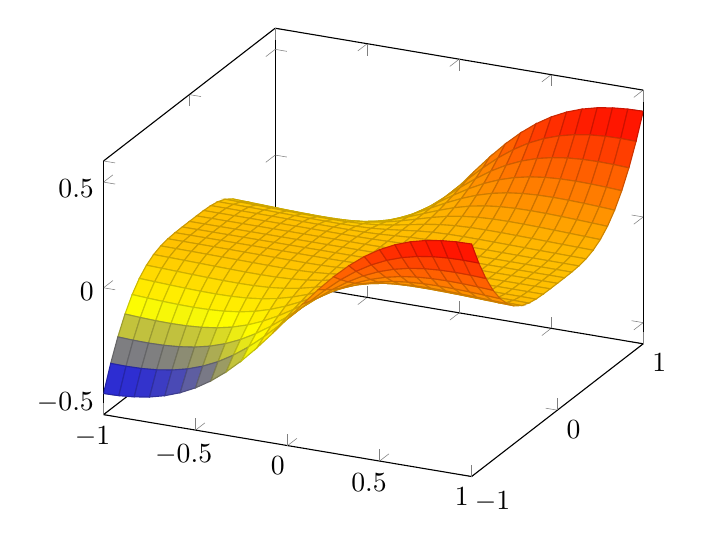
\begin{tikzpicture}
\begin{axis}[domain=-1:1,y domain=-1:1]
	\addplot3[surf] {\y^4*\x/(\x^2+\y^2)};
\end{axis}
\end{tikzpicture}
\end{center}
Graafikut moodustav kood:
\begin{verbatim}
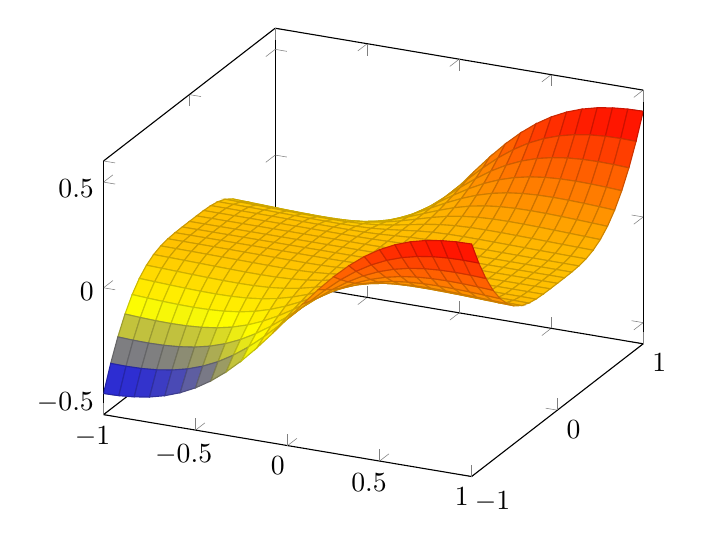
\begin{tikzpicture}
\begin{axis}[domain=-1:1,y domain=-1:1]
	\addplot3[surf] {\y^4*\x/(\x^2+\y^2)};
\end{axis}
\end{tikzpicture}
\end{verbatim}
\pagebreak
\textbf{3.} Arvutada kashe muutuja funktsiooni esimest järku Taylori valemi abil avaldise ligikaudne väärtus:
\begin{gather*}
(3,01)^2(0,97)^3.
\end{gather*}
Hinnata viga jääkliikme Lagrange'i kuju abil.\\
\textbf{Lahendus:}\\
Esimest järku Taylori jada üldkuju on $f(x,y)=f(P_0)+df(P_0)+\alpha_1$.\\
Kasutan funktsiooni $f(x,y)=x^2y^3$ algpunktiga $P_0=(3;1)$ ehk $dx=0,01$ ja $dy=-0,03$.\\
Leian funktsiooni osatuletised:
\begin{gather*}
\p{x}x^2y^3=2xy^3\\
\p{y}x^2y^3=3x^2y^2
\end{gather*}
Ehk $f$ täisdiferentsiaal on $df(x,y)=2xy^3dx+3x^2y^2dy$.\\
Leian Taylori valemiga ligikaudse väärtuse:
\begin{gather*}
(3,01)^2(0,97)^3=f(3,01;\ 0,97)=f(3,1)+2x_0y_0^3dx+3x_0^2y_0^2dy+\alpha_1\\
=3^2+2\cdot 3\cdot 1^3\cdot 0,01+3\cdot 3^2\cdot 1^2\cdot(-0,03)+\alpha_1\\
=8,25+\alpha_1
\end{gather*}
Seega $(3,01)^2(0,97)^3\approx 8,25$.\\
Leian funktsiooni teist järku osatuletised:
Jääkliikme hinnang Lagrange'i kuju abil:
\begin{gather*}
\alpha_1=
\end{gather*}
\end{document}